\documentclass[journal=esthag,manuscript=article]{achemso}

% additional packages
\usepackage[utf8]{inputenc}
\usepackage{amsmath}
\usepackage{booktabs}
\usepackage{subcaption}
\usepackage{tabularx}
\usepackage{array,multirow,graphicx}
\usepackage{comment}
\graphicspath{
  {./../figures/},
  {./../figures/air-exchange-rate/},
  {./../figures/kde-iacc-pressure/},
  {./../figures/simulation_predictions/},
  {./../figures/pair_grids/},
  {./../figures/multivariate_analysis/}
}
\usepackage{lineno}
\linenumbers
% macros

% authors
\author{Jonathan G. V. Ström}
\affiliation[Brown University]{Brown University, School of Engineering, Providence, RI, USA}
\author{Yijun Yao}
\affiliation[Zhejiang University]{Zhejiang University, Hangzhou, China}
\author{Eric M. Suuberg}
\email{eric_suuberg@brown.edu}
\affiliation[Brown University]{Brown University, School of Engineering, Providence, RI, USA}

% title
\title{Transient Variability In Vapor Intrusion And The Factors That Influence It}

% keywords
\abbreviations{VI}
\keywords{Vapor intrusion, Preferential pathways, Temporal variability, Factor analysis, Modeling}

\begin{document}

\begin{abstract}

\end{abstract}

\section{Introduction}

Long term vapor intrusion (VI) studies in both residential and larger commercial structures have raised concerns regarding significant observed transient behavior in indoor air contaminant concentrations\cite{u.s._environmental_protection_agency_oswer_2015,folkes_observed_2009,holton_temporal_2013,johnston_spatiotemporal_2014,hosangadi_high-frequency_2017,mchugh_recent_2017,u.s._environmental_protection_agency_assessment_2015}.
VI involves the migration of volatilizing contaminants from soil, groundwater or other subsurface sources into overlying structures. VI has been a recognized problem for some time, but many aspects remain poorly understood, particularly with respect to the causes of large temporal transients in indoor air concentrations.
There is uncertainty within the VI community regarding how to best develop sampling strategies to address this problem\cite{u.s._environmental_protection_agency_oswer_2015,holton_temporal_2013,johnson_integrated_2016}. \par

Results from a house operated by Arizona State University (ASU) near Hill AFB in Utah, an EPA experimental house in Indianapolis, IN and a large warehouse at the Naval Air Station (NAS) North Island, CA have all shown significant transient variations in indoor air contaminant concentrations.
All were outfitted with sampling and monitoring equipment that allowed tracking temporal variation in indoor air contaminant concentrations on time scales of hours.
All have shown that these concentrations varied significantly with time - orders of magnitude on the timescale of a day or days.
\cite{holton_evaluation_2015,guo_vapor_2015,hosangadi_high-frequency_2017}. \par

In one instance the source of the variation was clearly established during the study; at the ASU house a field drain pipe (or “land drain”), which connected to a sewer system, was discovered beneath the house, and careful isolation of this source led to a clear conclusion that this preferential pathway significantly contributed to observed indoor air contaminant levels and their fluctuations\cite{guo_vapor_2015,guo_identification_2015}.
While in this case the issue of a contribution from a preferential pathway was clearly resolved, what it left open was a question of whether existence of such a preferential pathway to an area beneath a structure would always be expected to lead to large fluctuations in indoor air contaminant concentrations. \par

Similarly, a sewer pipe has recently been suggested to be a source of the contaminants found in the EPA Indianapolis house.
That site was also characterized by large indoor air contaminant concentration fluctuations\cite{mchugh_evidence_2017,u.s._environmental_protection_agency_assessment_2015}.
Sewer lines have been generally implicated as VI sources at several sites\cite{pennell_sewer_2013,mchugh_evidence_2017,roghani_occurrence_2018,riis_vapor_2010}.
A Danish study estimate that roughly 20\% of all VI sites in central Denmark involve significant sewer VI pathways\cite{nielsen_remediation_2017}.
Thus while the consideration of a role of possible sewer or other preferential pathways is now part of normal good practice in VI site investigation\cite{u.s._environmental_protection_agency_oswer_2015}, it is still not known whether the existence of such pathways automatically means that large temporal fluctuations are necessarily to be expected.
In some of these cited cases\cite{pennell_sewer_2013,riis_vapor_2010}, a sewer provided a pathway for direct entry of contaminant into the living space.
While potentially important in many cases, this scenario is not further considered here, where the focus is on pathways that deliver contaminant via the soil beneath a structure. \par

It is, however, now known that even absent a preferential pathway, there may be significant transient variation in indoor air contaminant concentrations at VI sites\cite{folkes_observed_2009,brenner_results_2010,johnston_spatiotemporal_2014}.
One example is a site at NAS North Island at which no preferential pathways have been identified.
Instead, a building at this site is characterized by significant temporal variations in indoor-outdoor pressure differential\cite{hosangadi_high-frequency_2017}.
It is believed that this is the origin of the observed indoor air contaminant concentration fluctuations at that site. \par

This paper investigates the sources of the temporal variation in indoor air contaminant concentrations in both the presence and absence of preferential pathways.
In this work, the latter scenarios are referred to as ”normal” VI scenarios, in which there is typically a groundwater source of the contaminant.
Specifically, we pose the question of just how much variation in indoor air contaminant concentration may be expected at  such normal  VI  sites vs. those characterized by preferential pathways.
The conditions required for preferential pathways to become significant contributors to temporal variations in indoor air contaminant concentrations are also explored, and the consequences for sampling strategies are also discussed.



\section{Methods}

\subsection{Statistical Analysis}

This paper heavily relies on statistical analysis of high resolution datasets from two well-studied VI sites, one near Hill AFB in Utah (called the ASU house) and another in Indianapolis, IN (simply called as such.)
Analysis is performed using the SciPy, NumPy, Pandas, and Seaborn Python packages.
Probability distributions of various parameters are constructed using the kernel density estimation (KDE) method\cite{altman_introduction_1992}, which is implemented in the SciPy package.

To begin to characterize transient behavior in indoor air contaminant concentrations, actual datasets are analyzed to establish common levels of variability at VI sites.
For this purpose, the datasets from the ASU house in Utah, the EPA Indianapolis site and North Island NAS were chosen for analysis.
This paper relies on statistical analysis of published field data, and readers are referred to the original works for details regarding data acquisition\cite{holton_evaluation_2015,guo_vapor_2015,holton_temporal_2013,hosangadi_high-frequency_2017,u.s._environmental_protection_agency_assessment_2015}. \par

The ASU house data were obtained over a period of a few years.
During part of this time, controlled pressure method (CPM) tests were being conducted, in which the house was underpressurized to an extent greater than that characterizing “normal” operation.
This caused greater than normal advective flow from the subsurface into the house, thus increasing VI potential\cite{mchugh_evaluation_2012,mchugh_recent_2017,holton_evaluation_2015}.
This period of CPM testing is considered separately from the otherwise ”natural” VI conditions in the analysis.
Likewise, the existence of a preferential pathway at the ASU house needs to be considered in examining the dataset, noting that during some of the testing, this pathway was deliberately cut off, resulting in what we have termed “normal” VI conditions in which the main source of contaminant was believed to be groundwater. \par

The NAS North Island dataset has not (as far as is known) been influenced by a preferential pathway, but the structure there was subject to large internal pressure fluctuations, much more extensive than those typically recorded at the ASU house during normal operations.
Additionally, the underlying soil at NAS North Island is sandy and more permeable than that at the ASU site, which, as will be shown, contributes to the indoor air contaminant concentrations being more sensitive to pressure fluctuations\cite{hosangadi_high-frequency_2017}. \par

Likewise, the Indianapolis site investigation spanned a number of years and periodically included the testing of a sub-slab depressurziation system (SSD).
The goal of the SSD testing was to mitigate the VI risk by drastically depressurizing the sub-slab area underneath the house, preventing the contaminants from entering the structure above.
Only the period before the installation of this system was considered in the present analysis.
It is likely a sewer line beneath the structure acted as a preferential pathway\cite{mchugh_evidence_2017}, however at no point was this preferential pathway removed, making it difficult to assess how significant the role of the preferential pathway was at this site.
Regardless of this it is of interest to consider the data from this site due to how extensive and complete the data collection was. \par

The typical variation in indoor air contaminant concentrations with time will first be considered below in the case of the ASU house during ”natural”, (i.e. non-CPM conditions), in the case of the NAS North Island site over the entire available dataset, and for the Indianapolis case we consider the variations before the installation of the SSD system.
The deviations in indoor air concentration from the mean TCE (and Chloroform and PCE at the Indianapolis site) values, as well as the indoor-outdoor pressure differentials associated with these concentrations were examined.
Both univariate and bivariate kernel density estimations (KDE) were constructed.
KDE is a technique that estimates the probability distribution of a random variable(s) by using multiple kernels, or weighting functions, and in this case, Gaussian kernels are used to create the KDEs.
This means that it is presumed that the variables of interest (i.e., indoor air contaminant concentrations and indoor-outdoor pressure differentials, as sampled) are normally distributed around mean values (and that there are statistical fluctuations associated with each sampling event).
In this instance, the scipy statistical package was used to construct the KDEs, assuming a bandwidth parameter determined by Scott's rule.
The distributions of the individual parameters and the relationship between them will be examined using the KDE method.

\subsection{Vapor Intrusion Model}



\section{Results \& Discussion}

\subsection{Statistical Analysis of Field Data}



\begin{figure}[!h]
		\centering
    \caption{ }
    \label{fig:pair_grid}
    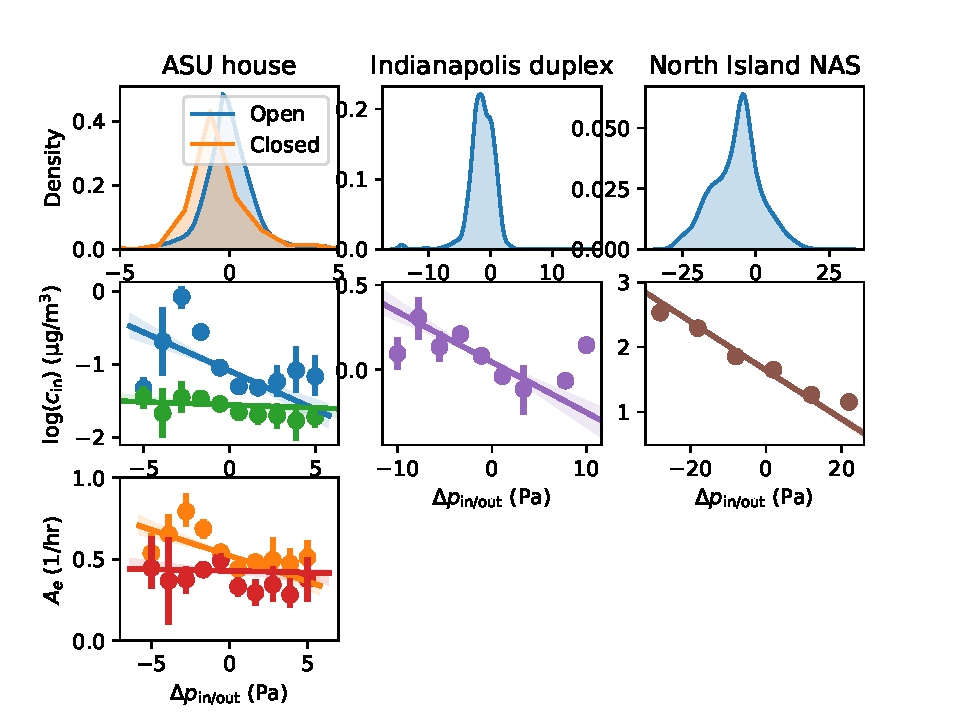
\includegraphics[width=\textwidth]{simple_grid.pdf}
\end{figure}

\begin{figure}[!h]
	\centering
	\begin{minipage}[c]{0.49\textwidth}
		\centering
    \caption{ }
    \label{fig:resampling}
    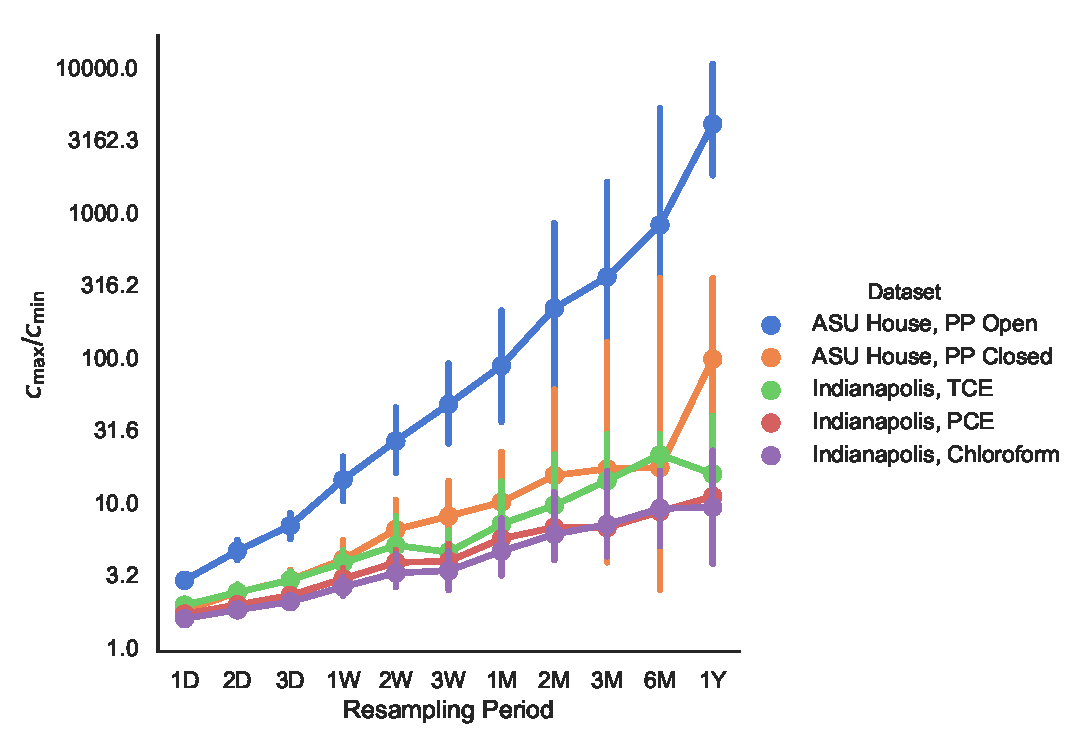
\includegraphics[width=\textwidth]{temporal_variability/resampling.pdf}
	\end{minipage}
	%\hspace{3cm}
	\begin{minipage}[c]{0.49\textwidth}
		\centering
    \caption{Simulated cases}
    \label{fig:land_drain_scenarios}
    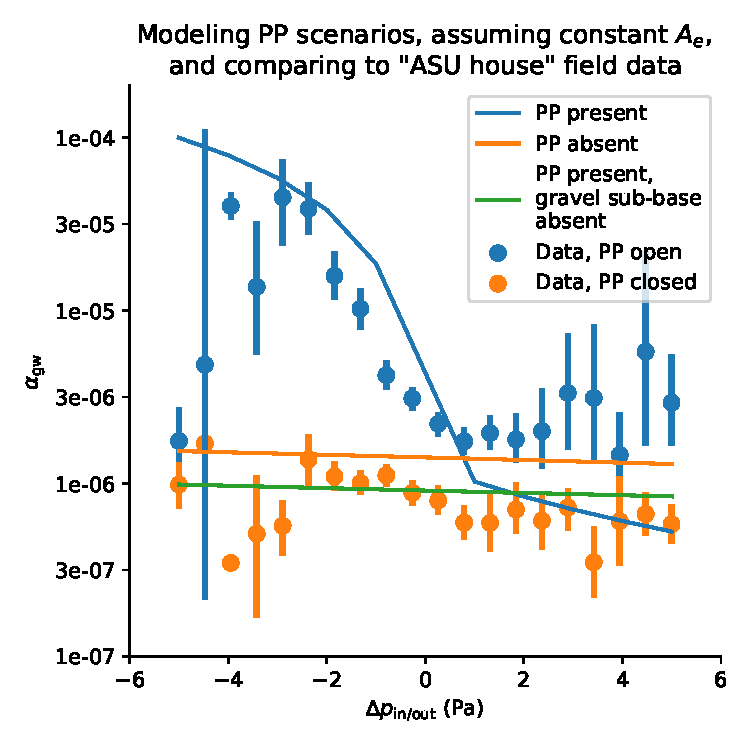
\includegraphics[width=\textwidth]{land_drain_scenarios.pdf}
	\end{minipage}
\end{figure}



\subsubsection{Modeling Indoor Air Variability}

\begin{figure}[htb!]
  \caption{ }
  \label{fig:simulation_sampling}
  % ASU/North Island plot
  \begin{subfigure}{0.49\textwidth}
    \centering
    \caption{ }
    \label{fig:simulation_sampling_pp_open}
    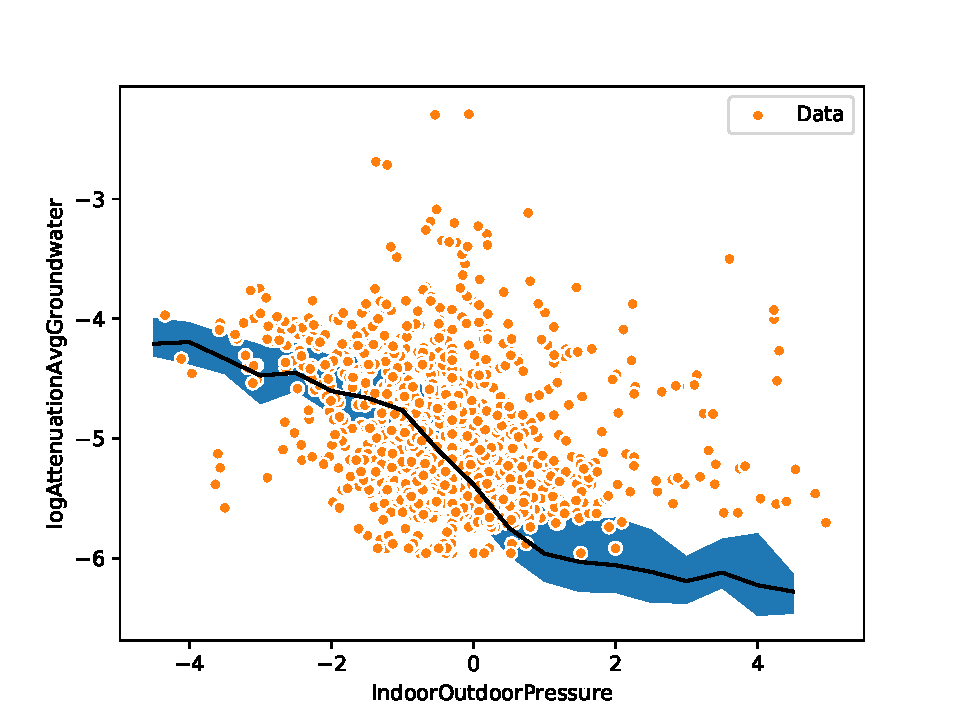
\includegraphics[width=\textwidth]{simulation_prediction_span_open.pdf}
  \end{subfigure}
  % Indianapolis plot
  \begin{subfigure}{0.49\textwidth}
    \centering
    \caption{ }
    \label{fig:simulation_sampling_pp_closed}
    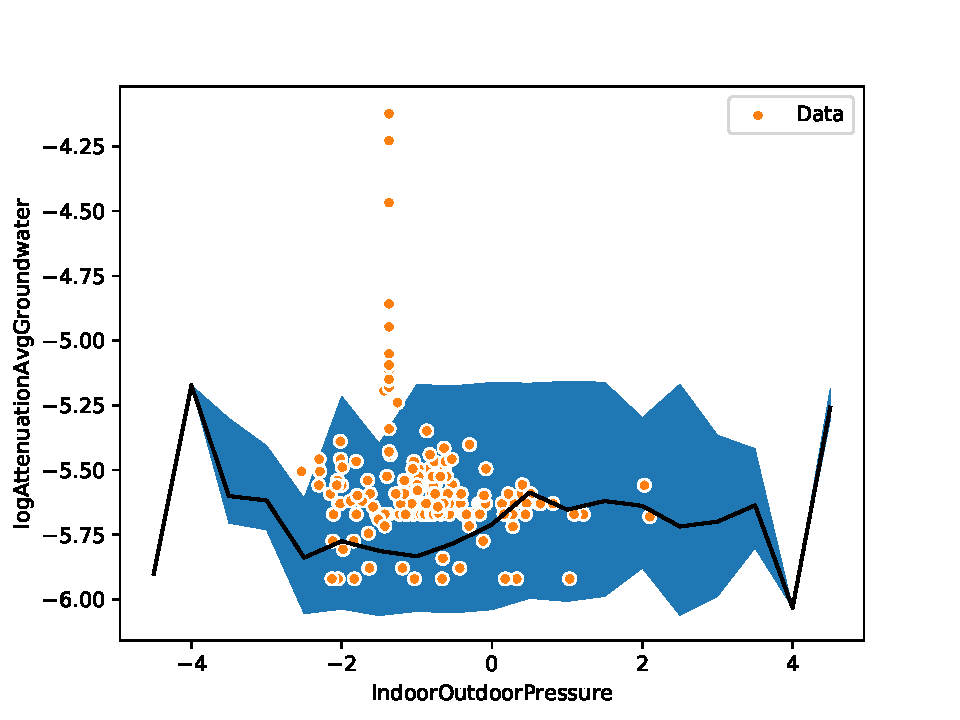
\includegraphics[width=\textwidth]{simulation_prediction_span_closed.pdf}
  \end{subfigure}
\end{figure}


\begin{acknowledgement}
  This project was supported by grant ES-201502 from the Strategic Environmental Research and Development Program and Environmental Security Technology Certification Program (SERDP-ESTCP).
\end{acknowledgement}

\bibliography{library}

\end{document}
